\chapter{Experimentos}

%El título del capítulo es flexible de acuerdo a cada tesis. Algunos títulos sugeridos podrían ser:
%\begin{itemize}
%\item El algoritmo X: nuestra propuesta.
%\item La técnica Y
%\end{itemize}
%Este título debe de estar ade acuerdo con el asesor del tema. Consúltelo en su sala de clase.

En este capítulo explicaremos la información necesaria y los procedimientos seguidos para llevar a cabo la experimentación. En primer lugar se explicarán los conjuntos de datos que servirán de base y referencia para los experimentos; luego se detallarán algunos detalles de la metodología; y finalmente se explicarán los experimentos a seguir.

\section{Conjuntos de datos}

Los conjuntos de datos que serán utilizados como casos de prueba son los siguientes:

\begin{description}
    \item[Apurata] Conjunto de datos privado de la \textit{fintech} peruana con el mismo nombre
    \item[Lending Club] Conjunto de datos público de la mayor \textit{fintech} de préstamos peer to peer en EE.UU.
    \item[Crédito Alemán] Conjunto de datos público de entidades bancarias Alemanas
\end{description}

Una mejor comparación entre estos conjuntos se puede encontrar en la tabla \ref{tab:dataset-comparison}

\begin{table}
    \centering
    \caption{Conjunto de datos utilizados}
    \label{tab:dataset-comparison}
    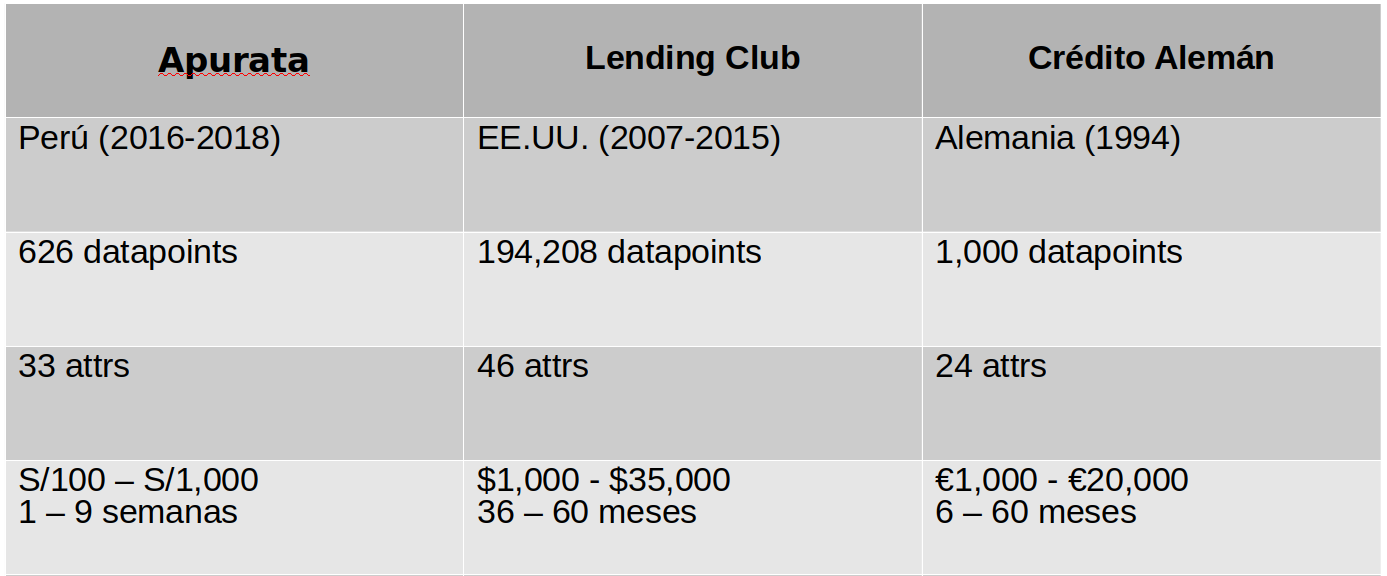
\includegraphics[width=0.8\linewidth]{graficos/dataset_comparison.png}
\end{table}

Como se puede apreciar, todos los conjuntos se componen de pocas características, ninguno de ellos supera las 50. Los conjuntos de datos de Apurata y del Crédito Alemán además son pequeños respecto a la cantidad de instancias, con 1000 o menos.

También se cumple que los 3 conjuntos de datos son desbalanceados, ya que la clase de ``Moroso", representa el 15\% para Apurata, 24\% para Lending Club y el 30\% para Crédito Alemán.

Por otro lado, los 3 conjuntos también poseen diferencias importantes entre sí que enriquecen su estudio. Apurata y Lending Club son \textit{fintech} que utilizan diferentes criterios de los de los bancos para seleccionar su información. Los conjuntos de Crédito Alemán y Lending Club registran créditos que se realizan por montos más altos y a un mayor plazo que los de Apurata. Los periodos de tiempo y los países abarcados por los conjuntos de datos también son únicos, y finalmente Lending Club tiene bastante más instancias que los otros 2 conjuntos.

Los conjuntos de Crédito Alemán y Lending Club son considerados referenciales en sus respectivos sub-dominios, ya que hay varios estudios que los utilizan para realizar sus experimentos. Entre los que usan los datos de Lending Club tenemos \citep{malekipirbazari2015risk, zhang2016research, zang2014credit, tan2018deep}. Y entre los que usan los datos del Crédito Alemán tenemos \citep{harris2015credit, nanni2009experimental, brown2012experimental, wang2012two}.

\section{Metodología}

Para el preprocesamiento de la información, se eliminaron las variables con más del 50\% de información faltante, luego se eliminaron las filas con información faltante. A las variables resultantes se les convirtió a variables numéricas; y finalmente se hizo una normalización entre -1 y 1.

La interpretación de la variable $y$ se hizo de la siguiente manera: 1 para los buenos pagadores y 0 para los malos.

Para la selección de parámetros se realizó un grid-search con un ajuste fino manual al final. Sobre el desbalanceo de los datos, no se tomó ningún procedimiento especial. 

Para evaluar el desempeño de los modelos se hizo 10-fold validation 10 veces en Apurata y en el Crédito Alemán y 1 sola vez en Lending Club, ya que tiene abundantes datos. Finalmente se extrajo el promedio de todas las mediciones como la medición final. 

Las métricas utilizas son la exactitud, la precisión, la exhaustividad y el \ac{AUC}. La métrica que se buscó optimizar fue el \ac{AUC}. Para las otras métricas se tuvo que seleccionar un punto de corte óptimo, que se escogió tratando de optimizar la exactitud, de modo que los resultados son comparables con el estado del arte.

\section{Experimentos}

En esta sección se describirán los experimentos llevados a cabo.

\subsection{Experimento 1}

El primer paso es hacer una comparación entre los clasificadores individuales y los \ac{ECDD}. El objetivo de este experimento es verificar si efectivamente el desempeño mejora individualmente por cada clasificador, sin hacer una comparación transversal entre clasificadores de distintas familias.

En este experimento también evaluaremos la posibilidad de usar un algoritmo de aprendizaje profundo: \ac{DBN}.

\subsection{Experimento 2}

En este experimento compararemos los \ac{ECDD} con dos algoritmos de bagging usados ampliamente en la actualidad: \ac{RF} y \ac{XGBoost}. El objectivo de este experimento es verificar que el método de \ac{ECDD} es competitivo con otros métodos de ensamble del estado del arte, sin el sesgo de haber usado una metodología diferente para el entrenamiento y la evaluación de los modelos.

\subsection{Experimento 3}

Finalmente en el experimento 3 compararemos los resultados obtenidos por nuestros \ac{ECDD} con los resultados obtenidos en otros estudios del estado del arte que usan los mismos conjuntos de datos. El objetivo de este experimento es ratificar que los resultados son válidos para el estado del arte usando dos conjuntos de datos referenciales.
